\section{Initial problem} %initial problem
At the beginning of this project we were given a project-catalog, where we chose 'Vagtplanlægning' ('Work scheduling') as out subject. We had to delineate and define a problem. Luckily, a member of our group have a parent who works at \siemens, in a position with the function of creating the work schedule. She has to spend about a day on creating it, assuming it gets approved. If it does not, she will have to spend another whole day creating it from the bottom again. We chose this as a problem, since it is a real-life case, along with the possibility to get relevant people to actually user-test our solution, and compare it with what has been done previously.

We also made use of a Wh-diagram to narrow down our problem delineation. It has proven to quite a useful tool since it helped us understand the most important factors to take into account regarding our topic. In the end we were left with two possible problem delineations, focusing on improving the work scheduling to help the employer or doing it for the employee. As stated in our problem delineation, we chose to focus on the employee and making the schedule as fair as possible. There is no doubt the Wh-diagram has been particularly useful in that scenario, since it helped give us an overview of the interested parties as well as other important factors.

One of the most important factors we took into account when deciding on this topic, was that we wanted to work with a more authentic case instead of a purely theoretical one. That way we would also gain some practice when it came to working with real life problems, as we will be doing in future projects, for example our third semester project.

\section{From problem analysis to solution development}
The main purpose of the problem analysis was of course to get an understanding of \siemens's needs and understand the different interested parties as well as the definition of a fair schedule. The transition from working on the problem analysis to the solution development, since we had a solid foundation of knowledge upon which we could create our solution. It has therefore been quite easy to first and foremost outline the priorities of our program, since we only had about a month to create our program. 

One thing we did not do properly, regarding the use of our problem analysis in our solution development, was that we hardly used the analysis of existing solutions. Despite our research into already well functioning programs, we did not actually take these into consideration when developing our program. Another time we should probably go a bit more in depth of the analysis of different programs, look into their features and possible distinct advantages/disadvantages, and use that knowledge when creating our own program. However, the overall transition has been very smooth, and we have definitely experienced that the problem analysis has been very useful.
\begin{figure}[ht!]
    \centering
    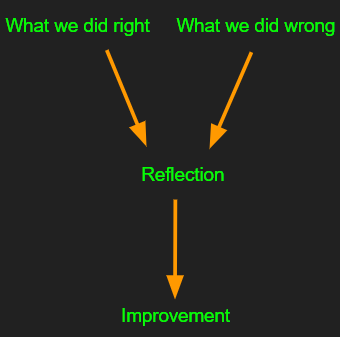
\includegraphics[width=5cm]{media/Gamma.PNG}
    \caption{The Gamma model: How we have worked in our process analysis}
    \label{fig:Gamma}
\end{figure}